\subsection{Track Trigger System Architecture}


\subsubsection{Tracker geometry and Trigger Towers }

\noindent 

Multiple challenges must be faced at the different stages of the processing chain.  First, data needs to be transferred out of the Tracker at the necessary speed.  Stubs from thousands of silicon modules must then be formatted, organized into $\eta-\phi$ trigger towers, duplicated and shared across tower boundaries as needed.  Next, pattern recognition and track fitting must be performed.  Finally, all reconstructed  tracks must be processed to form an intelligent trigger decision. A coherent system design for a Level-1 track trigger must consider each of these aspects.

For simplicity, we assume that the FEDs are upstream, receive fibers from the modules, and pass the relevant stub data to the track trigger system.  One could further consider an architecture in which the FED resides in the same ATCA shelf as the track trigger processing boards; however, the focus of this document is the Vertical Slice Demonstration System, not DAQ readout, so do not attempt to specify FED details here.
The FED interface will need to be defined for demonstration purposes, however the actual FEDs do not need to be involved in the tracking trigger demonstration.


\noindent The found stubs are sent from the modules using a block synchronous data transfer scheme which tolerates random occupancy fluctuations while bonding latency. The current plan is to have the data from 8 consecutive beam crossings as one block. The front-end designers are finalizing the baseline of the data formats after much work investigating different format variants for robustness against rate fluctuations, ease of implementation, impact on power consumption, etc. While choosing the 8 crossings scheme as our current working assumption, our strategy is to design the downstream components to be flexible enough to handle different possible formats. 


\begin{figure}[ht!]
\centering
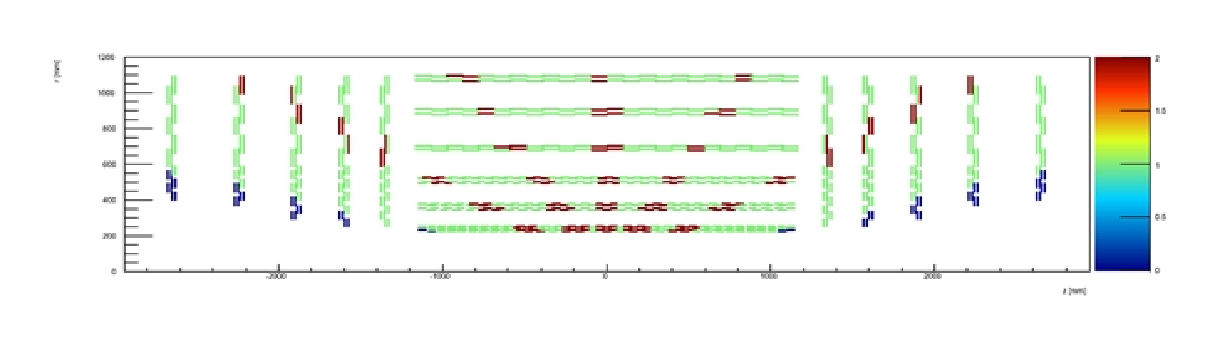
\includegraphics[width=0.75\columnwidth]{Plots/SecDef_RZ.eps}
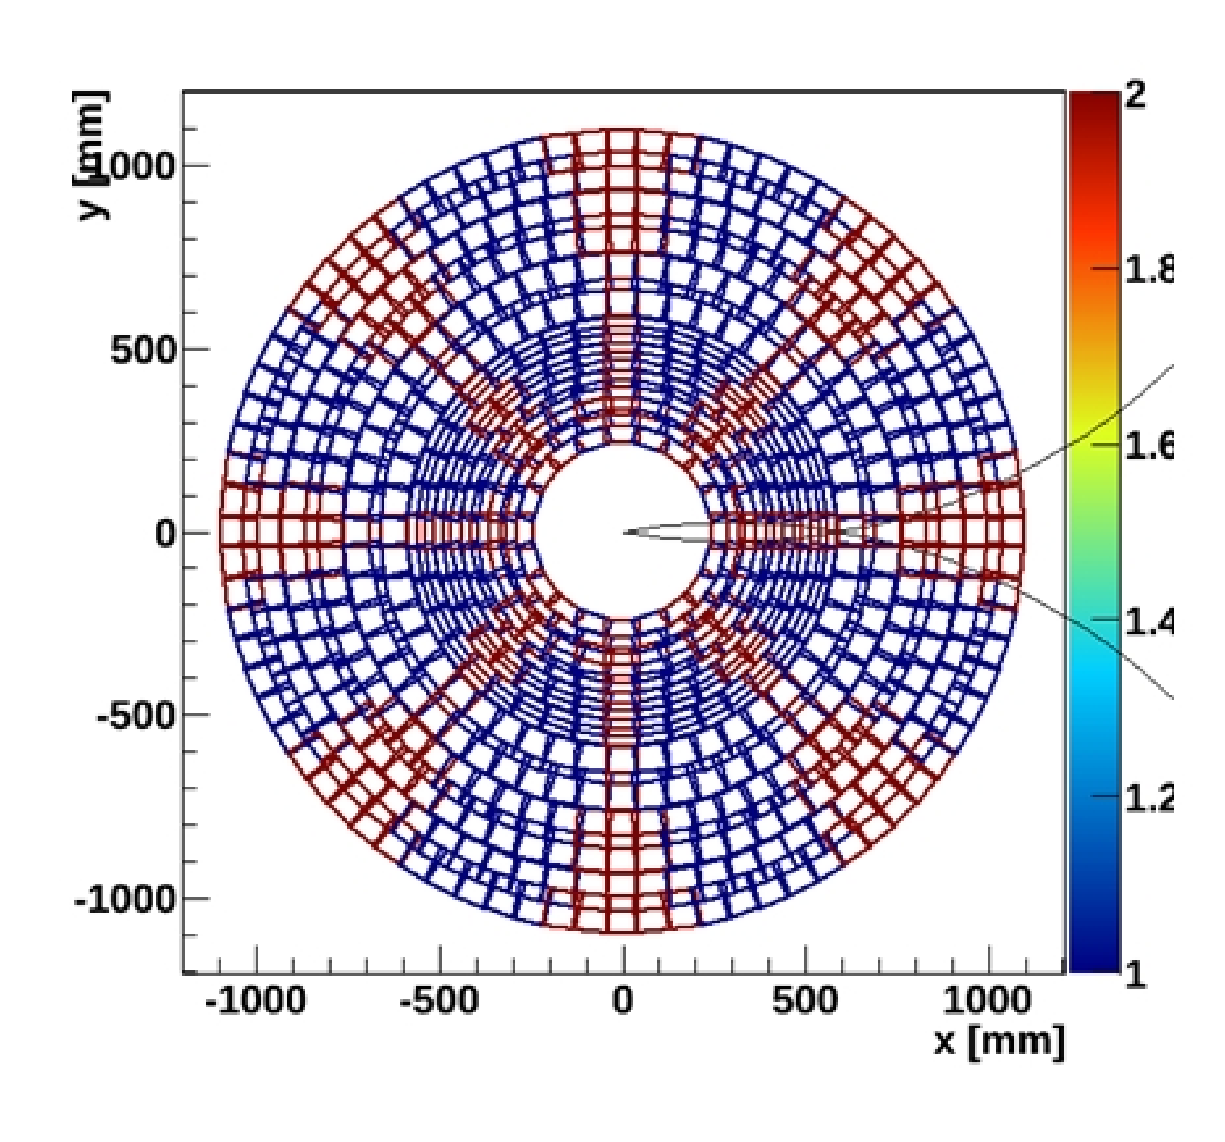
\includegraphics[width=0.2\columnwidth]{Plots/SecDef_XY.eps}
\caption{Six sectors in $\eta$ (left). Note that the symmetry around $\eta=0$ will provide for easier cable grouping. Eight sectors in phi (right).}
\label{fig:SecDef_RZ}
\end{figure}

\noindent 
Stubs from the 15K silicon modules must be delivered to the correct trigger towers.  Detailed data sharing studies have been performed for the Barrel-Endcap (BE) Tracker geometry with different trigger tower partitions.  Based on these studies, a 6 (in $\eta$) x 8 (in $\phi$) = 48 trigger tower partition has been chosen as the baseline configuration (see Figures~\ref{fig:SecDef_RZ}). Detailed studies have been performed on data sharing assuming the default 48 tower partition with a minimum $p_T$ of 2 GeV and track origin smearing in $z\pm 7$ cm. Figure~\ref{fig:TT_config} shows the number of trigger towers that stubs from a given module must be delivered to under these conditions. When a stub is in the middle of the trigger tower, it will have to be delivered to only one tower (to the native trigger tower). When a stub is near the boundary in phi or eta (but not both), it will have to be delivered to two towers. If a stub is at both the boundaries in eta and phi, it will have to be delivered to four towers. Note that four towers is the maximum number of towers any stub must be delivered to. 


\noindent The subdivision of the tracker into 48 trigger towers is shown in Figure~\ref{fig:TT_config} top, where the colored lines indicate all needed interconnections among the trigger towers. 
A unique feature of this arrangement is that any given trigger tower needs only to be connected with its immediate eight neighbors for stub sharing.  Studies have shown that this feature is essentially independent from the minimum pT threshold and track origin smearing in z. 

\begin{figure}[ht!]
\centering
%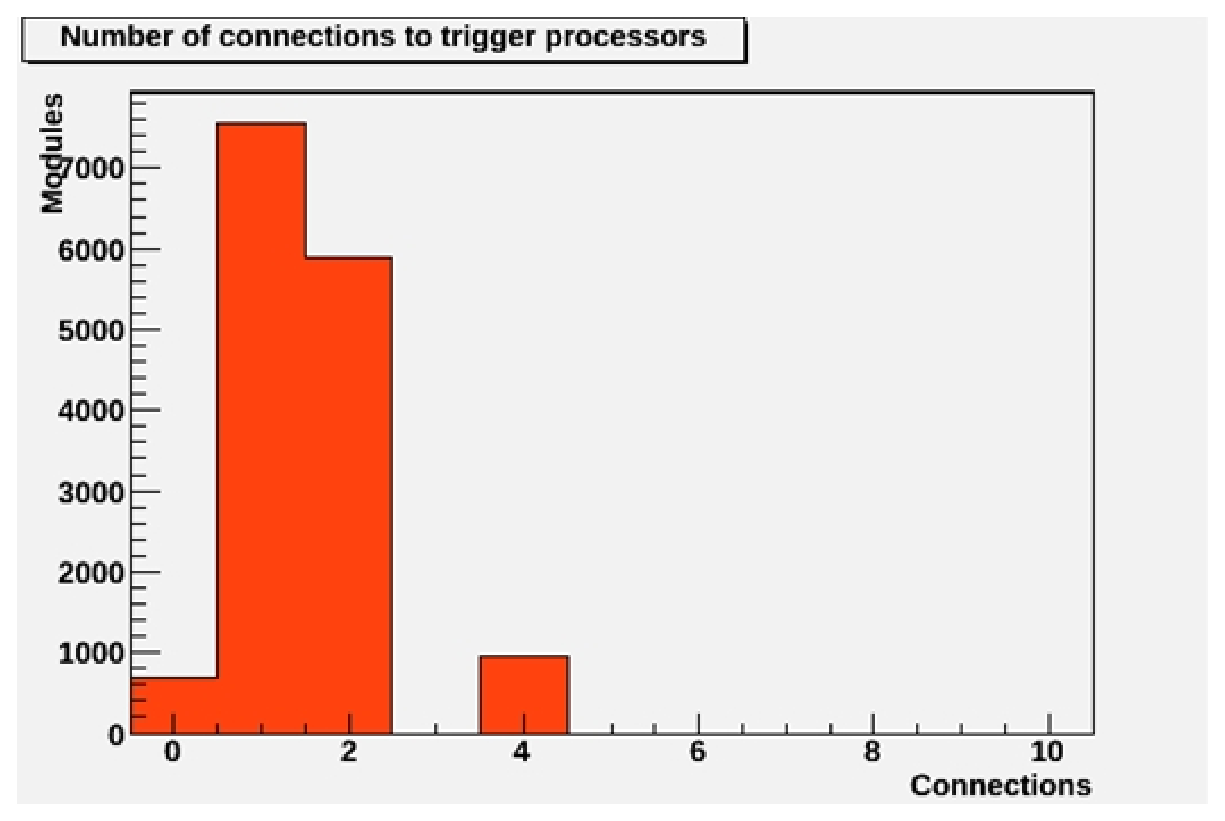
\includegraphics[width=0.45\columnwidth]{Plots/SecDef_N.eps}
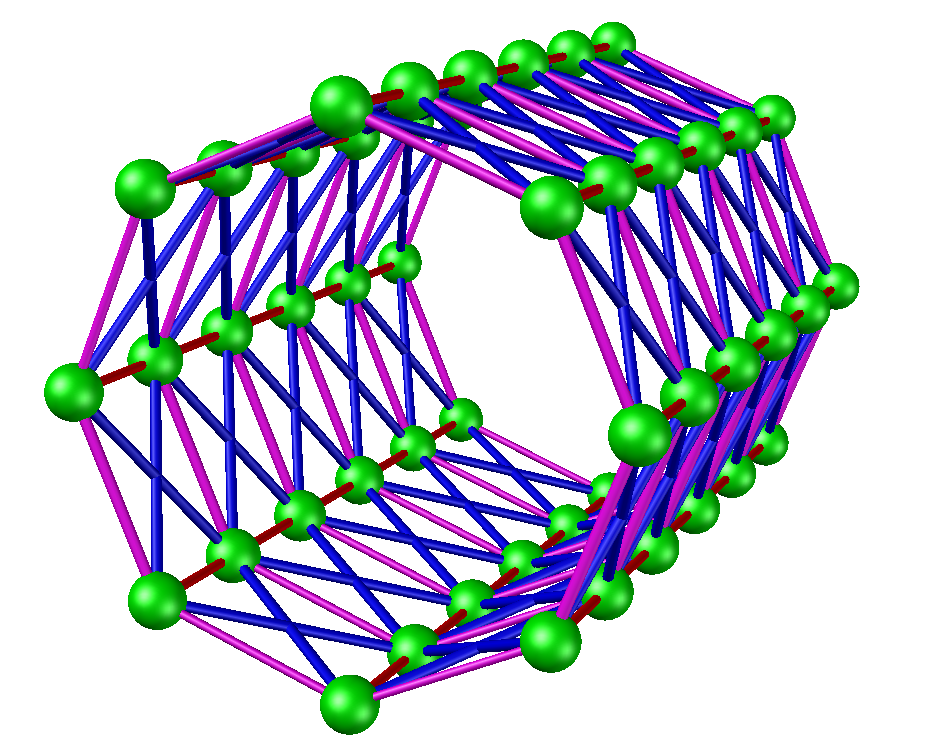
\includegraphics[width=0.4\columnwidth]{Plots/CMS_L1_48_towers.png}
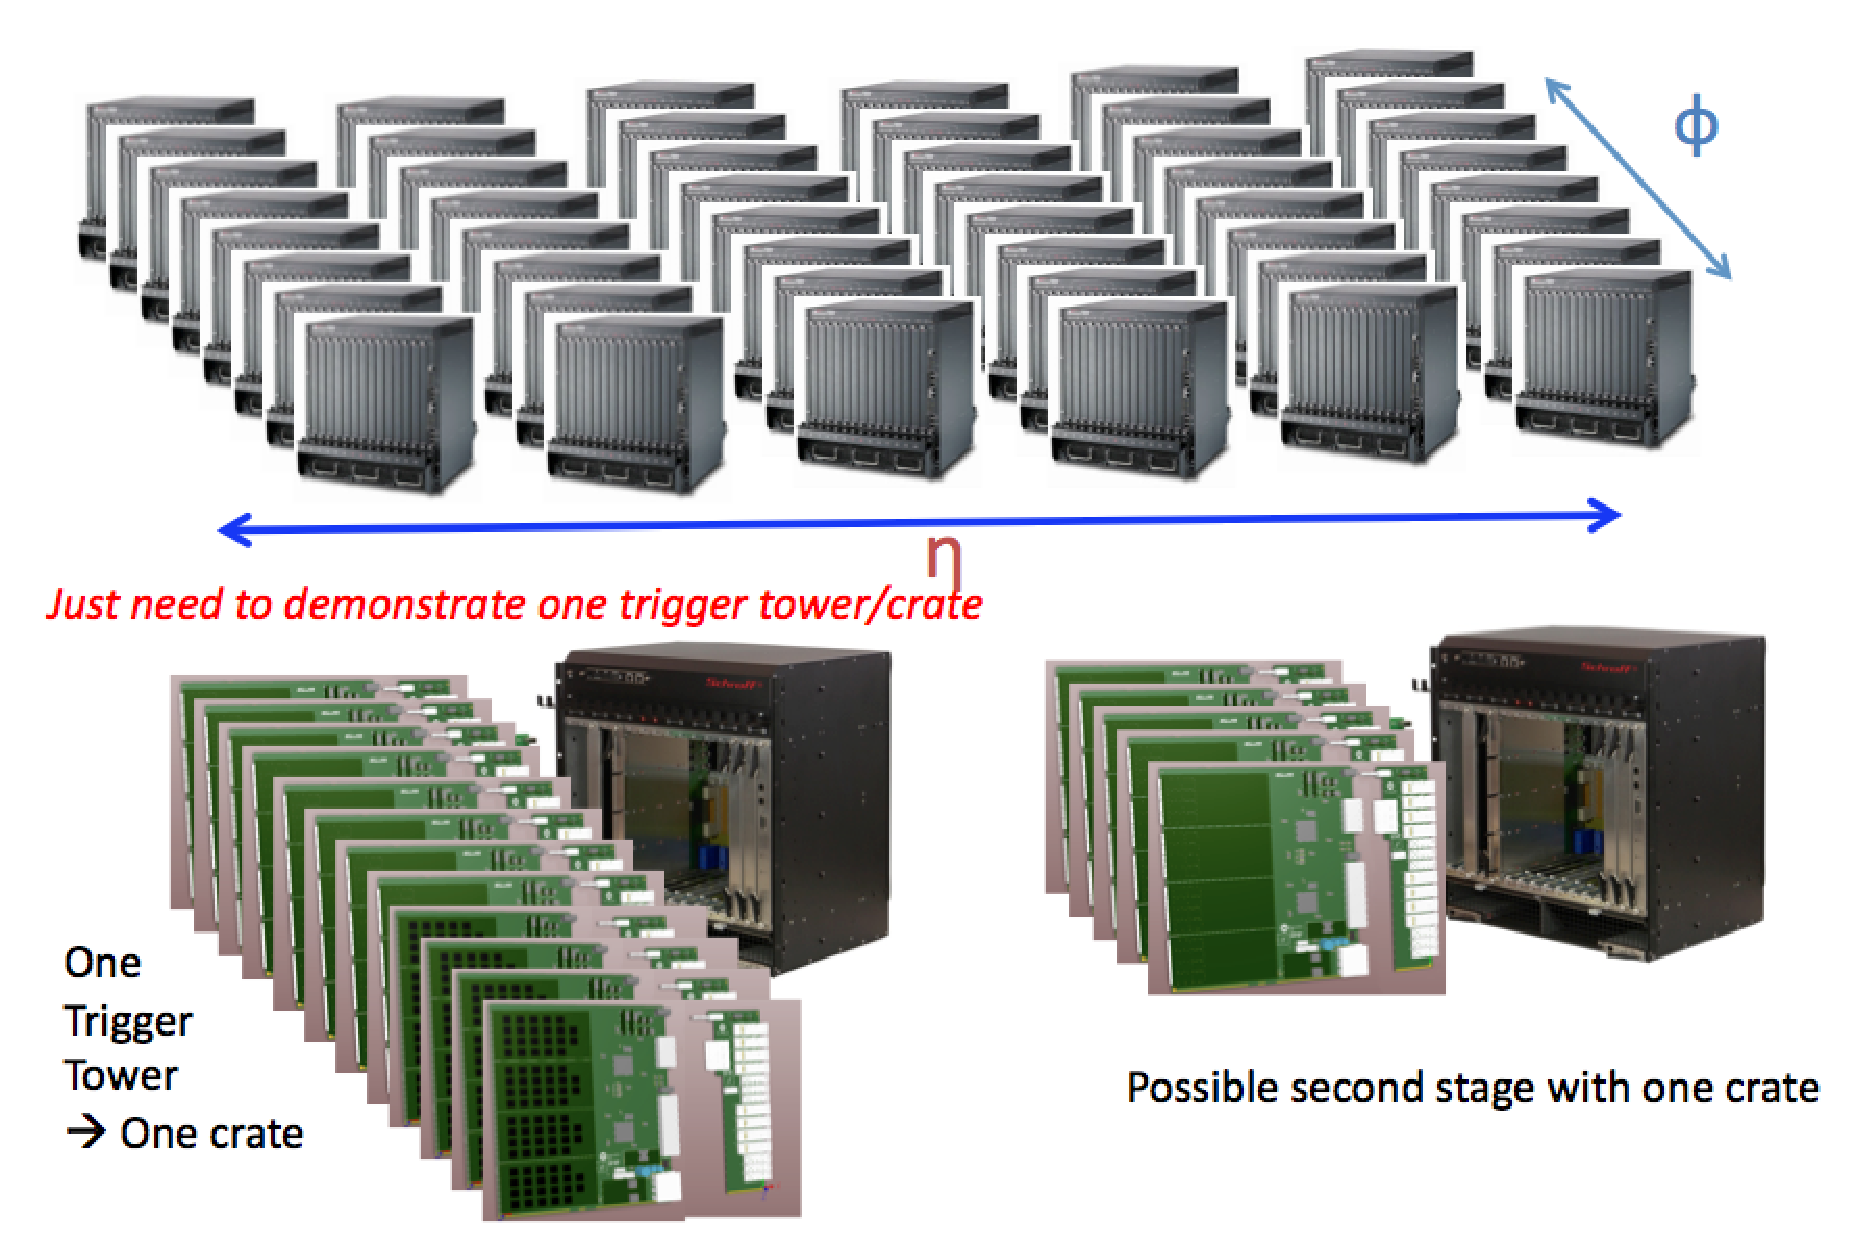
\includegraphics[width=0.7\columnwidth]{Plots/System_1.eps}
\caption{
Top: Conceptual view of the proposed CMS phase II L1 tracking trigger towers.  The formation is organized as 48 trigger towers (6 $\eta$ x 8 $\phi$).  Each node in this diagram represents a trigger tower processor engine.  Within each crate the full mesh backplane is used for time multiplexing of the incoming data, while the data sharing between towers is handled with inter-crate fiber links.
Bottom: 
A simple system configuration that can be built with today's technology assumes one 
ATCA shelf per trigger tower (the actual system will likely be smaller in the future).
}
\label{fig:TT_config}
\end{figure}

\subsubsection{System Architecture}

\noindent The tower processor platform must support large number of fiber transceivers, which are used for receiving input links and sharing data between neighboring towers.  A flexible, high bandwidth backplane is also required to quickly transfer data between boards.  The boards should be large enough to support pattern recognition engines and fiber connections. Given these requirements, we propose a full mesh 14 slot ATCA shelf to support the tower processors. An ATCA shelf is typically an air-cooled 13U rack mounted chassis consisting of 14 slots.  The first two slots are reserved for Ethernet switch blades.  Switch blades may include a fast CPU and are often used for controls and other system functions.  The remaining 12 slots are used for processor or payload blades.  In a full mesh ATCA backplane each pair of slots is directly connected with a multi-lane bidirectional serial channel capable of supporting sustained 40 Gbps data transfers.  A modern "40G" full mesh ATCA shelf has a total aggregate bandwidth of over 7 Tbps, not including external I/O.

\noindent 

For simplicity, we assume one ATCA shelf per trigger tower for the moment. Following this assumption, if the L1 Tracking Trigger system were built today, the full system would comprise 48 ATCA shevles, as shown in  Figs.~\ref{fig:TT_config}. Our assumption is, of course, very conservative.  The actual system will most likely be significantly smaller due to rapid progress in technology developement.
Note that connections between tower processor shelves are limited to eight nearest neighbors, and this can be easily achieved. 

In additon, as shown in Figure~\ref{fig:TT_config}, an additional shelf could act as a second stage processor.  Each board in this shelf could receive tracks from complete events, allowing track duplication removal to be implemented at this stage.  With more boards to sharing data over the full mesh backplane, it is also possible to implement jet related triggers, vertexing capabilities, track based MET calculations, etc.

%\begin{figure}[ht!]
%\centering
%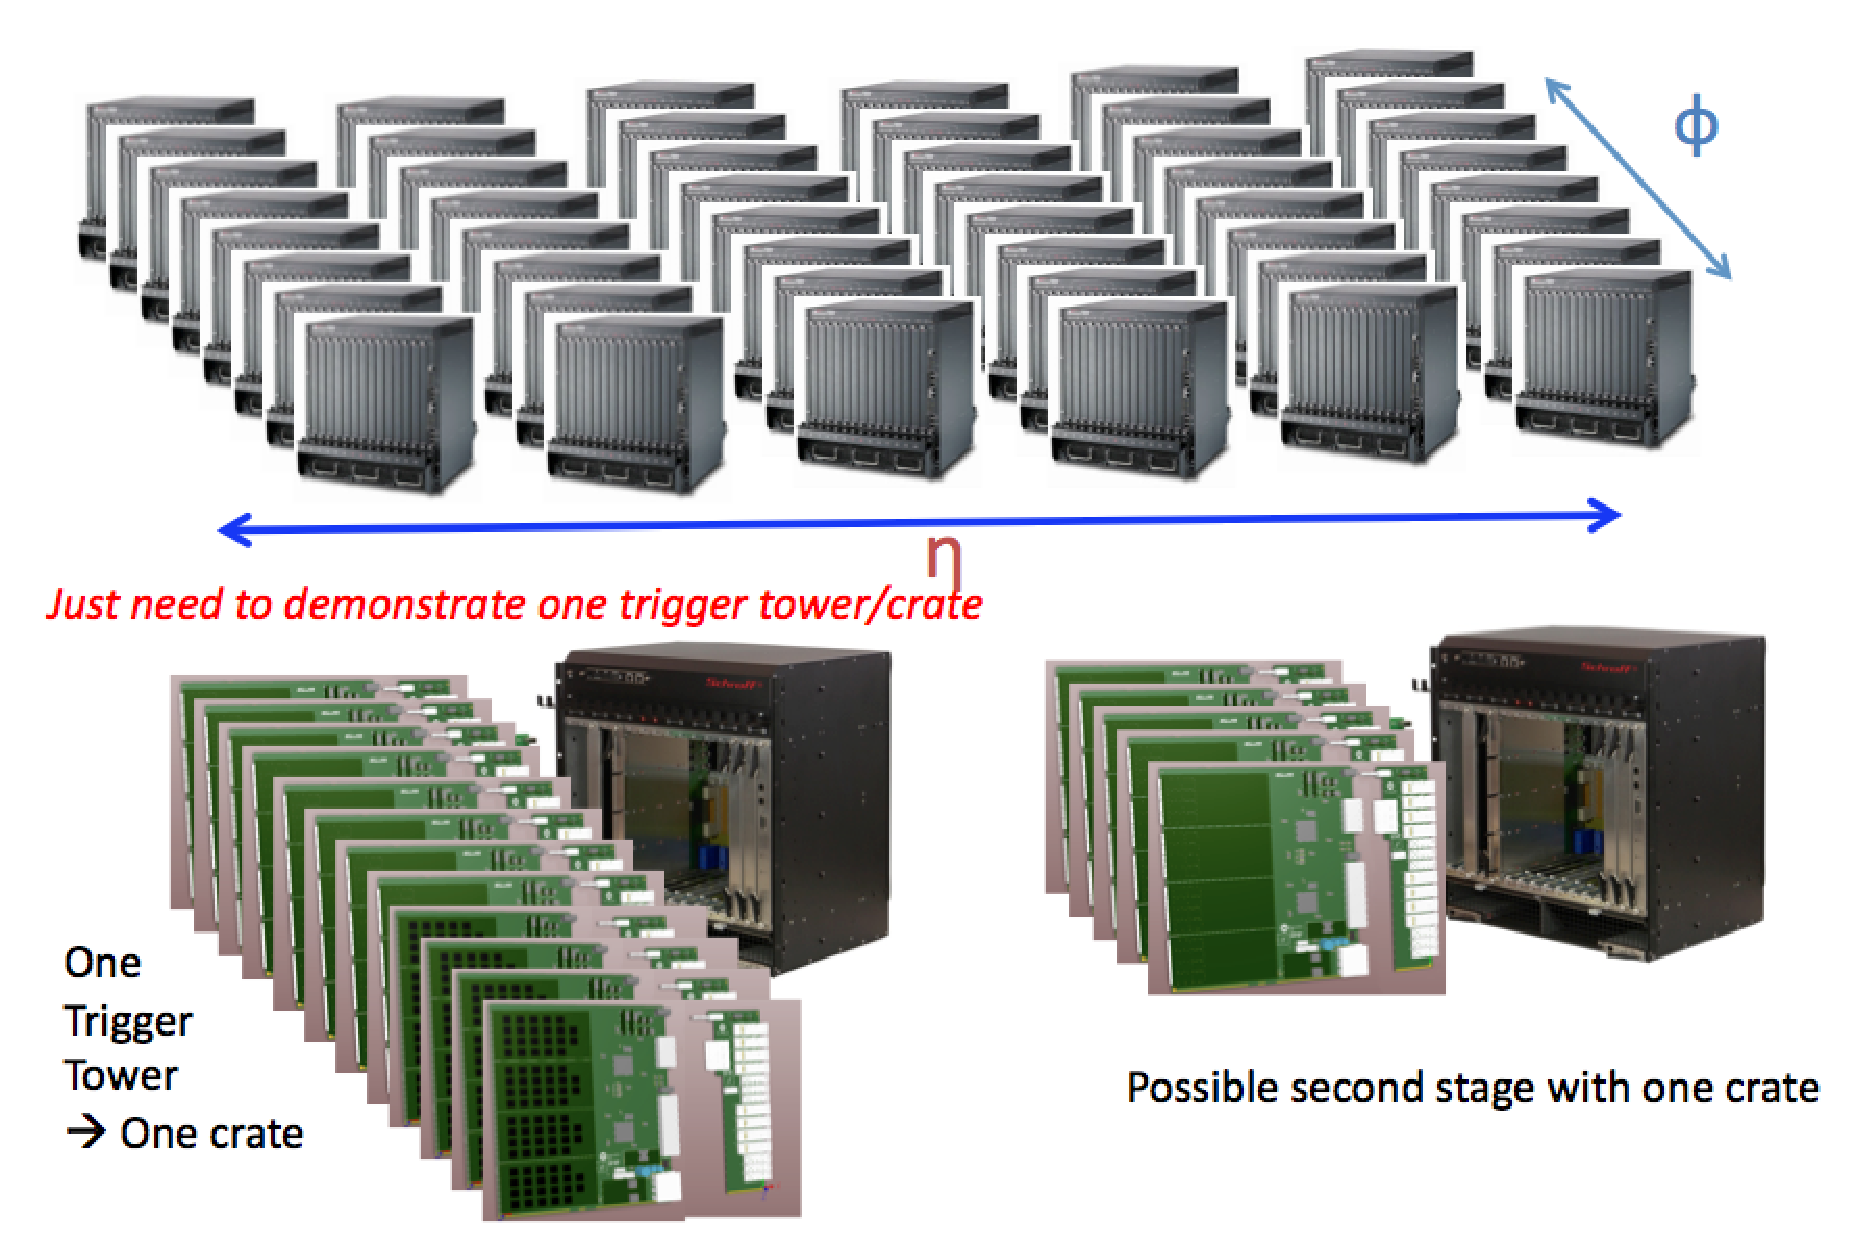
\includegraphics[width=0.7\columnwidth]{Plots/System_1.eps}
%\caption{Possible system configuration with today's technology by simply assuming one ATCA shelf per %trigger tower (the actual system will likely be smaller in the future)}
%\label{fig:System_1}
%\end{figure}

%\begin{figure}[ht!]
%\centering
%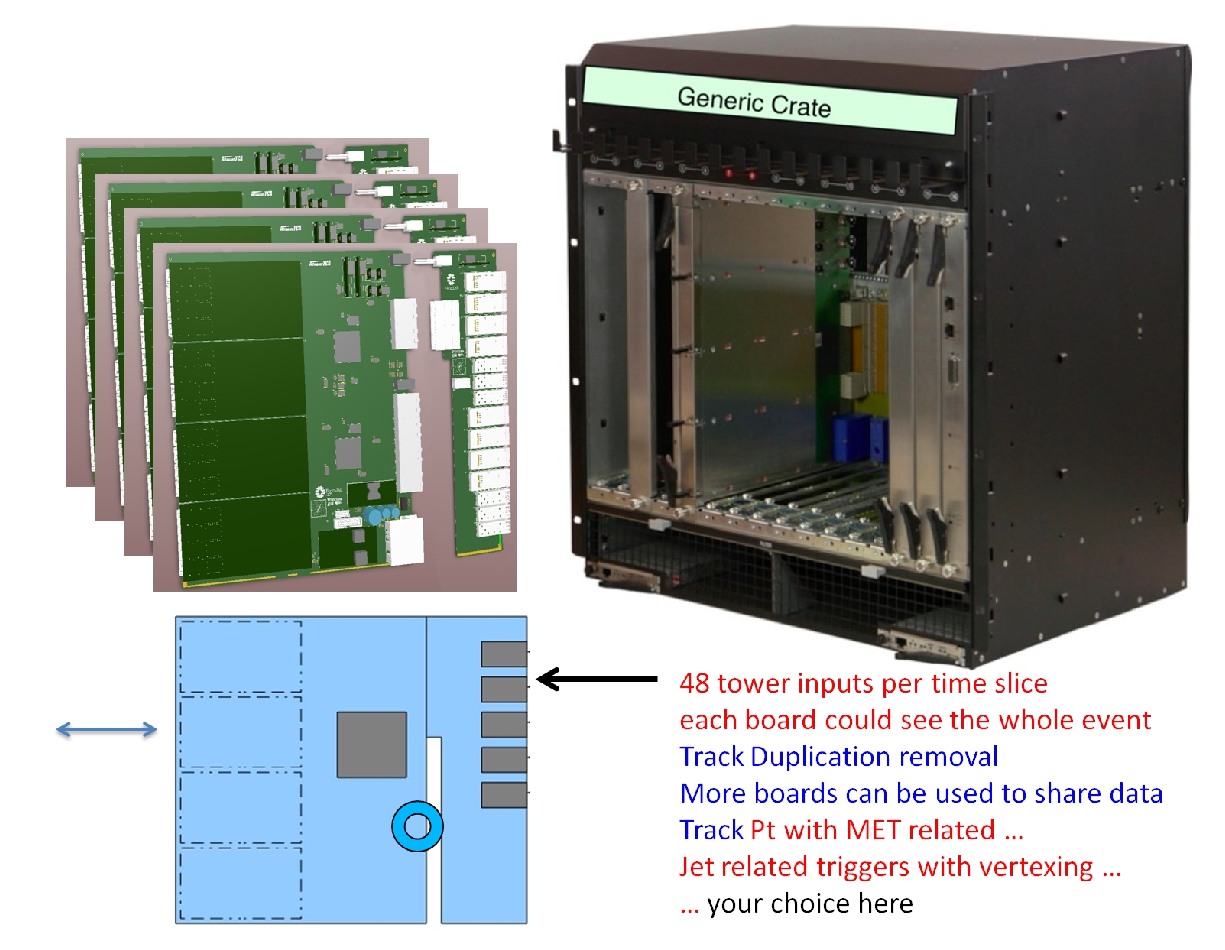
\includegraphics[width=0.5\columnwidth]{Plots/System_2.eps}
%\caption{The second processing stage shelf.}
%\label{fig:System_2}
%\end{figure}




%\begin{figure}[ht!]
%\centering
%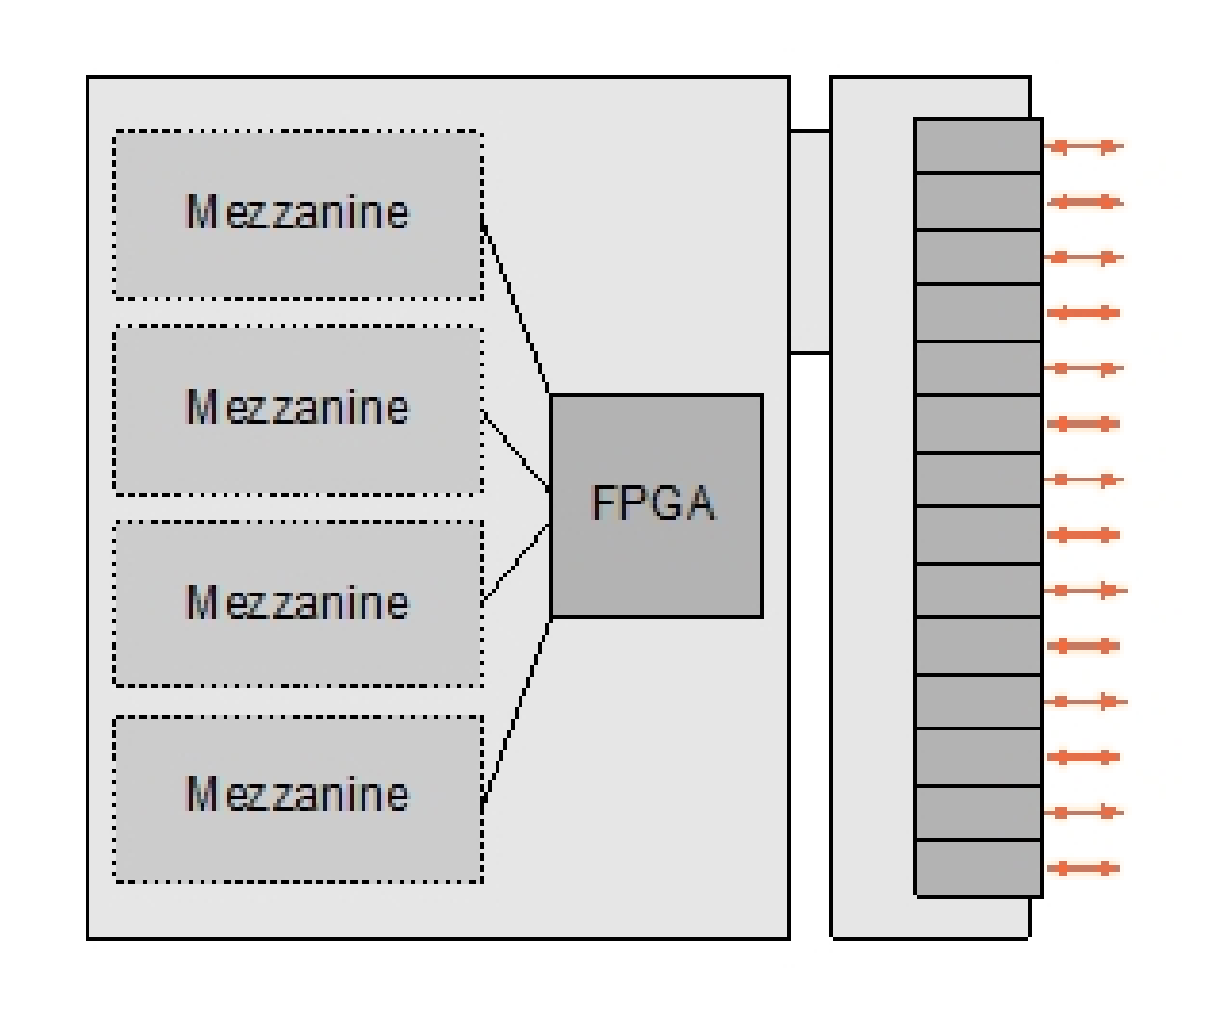
\includegraphics[width=0.4\columnwidth]{Plots/ProcBlade.eps}
%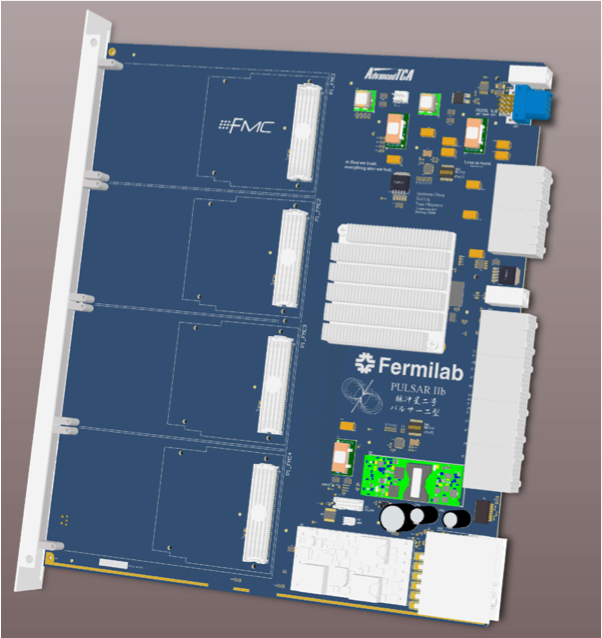
\includegraphics[width=0.4\columnwidth]{Plots/PulsarIIb.png}
%\caption{Generic processor blade concept (left), and the actual design of Pulsar %IIb~\cite{bib:PulsarII}~\cite{bib:PulsarII-weblink} at final layout stage (right)}
%\label{fig:ProcBlade}
%\end{figure}

%\begin{figure}[ht!]
%\centering
%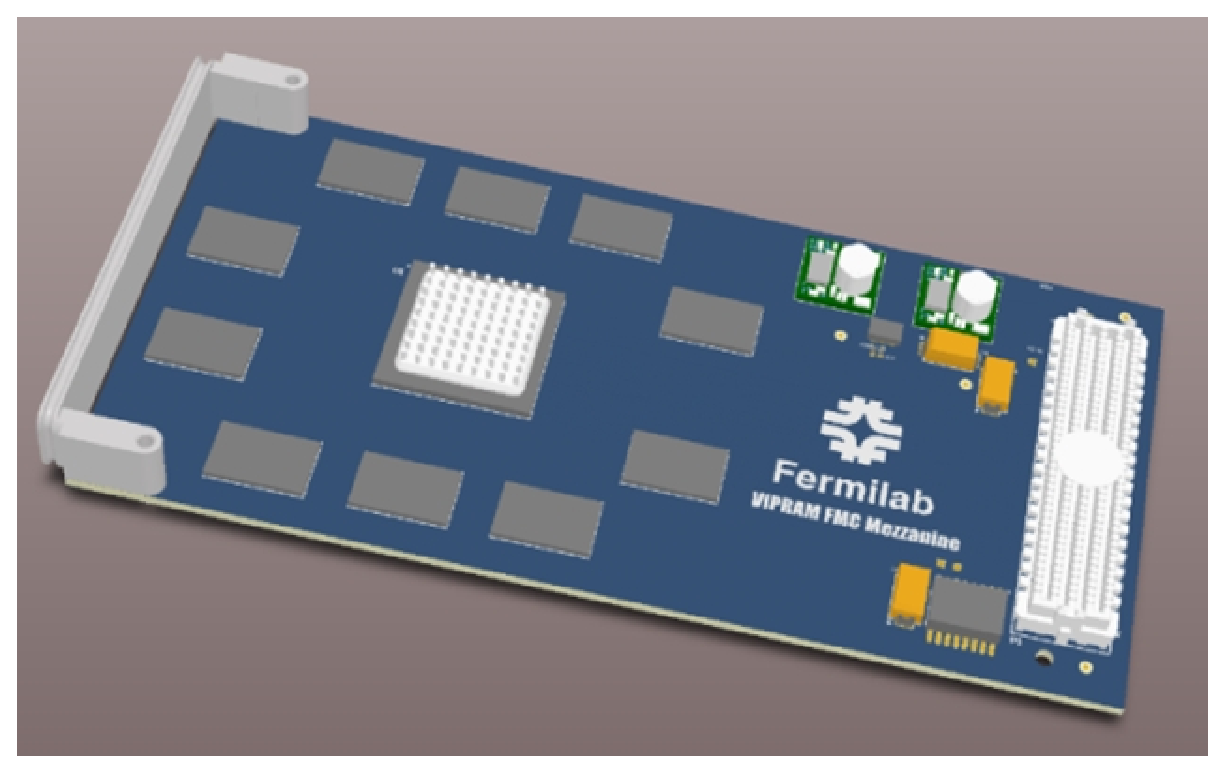
\includegraphics[width=0.4\columnwidth]{Plots/PRAM.eps}
%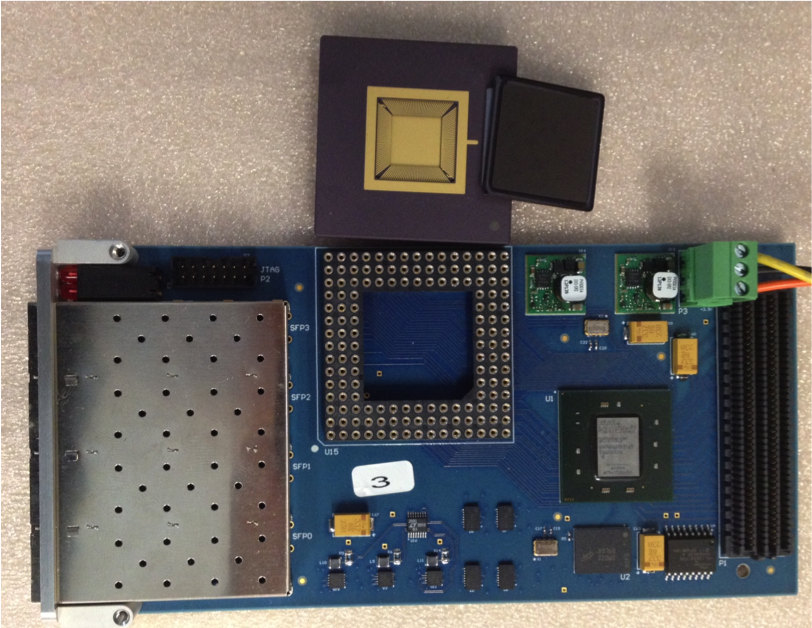
\includegraphics[width=0.4\columnwidth]{Plots/test_mezzanine.png}
%\caption{Left: Concept of a pattern recognition mezzanine design for testing different pattern recognition %algorithms.
%Right: a test mezzanine prototype designed and built at Fermilab, features four SFP+ pluggable serial %transceivers (for standalone
%data receiving), a Kintex 7 FPGA, configuration flash memory, DDR3 memory, power supplies, local %oscillators, a test socket for
%associative memory chips developed at Fermilab, and FMC connectors. 
%}
%\label{fig:PRAM}
%\end{figure}

\noindent The processor blade is the Pulsar 2b, which is shown in Figure~\ref{fig:ProcBlade}.  The front board measures 8U x 280mm and is designed around a single FPGA.  This FPGA connects directly to the full mesh backplane fabric, mezzanine cards, and fiber transceivers located on a rear transition module (RTM).  For the most part, communication channels are high speed serial point to point links and are directly supported by SERDES transceivers in the FPGA. 

\noindent The fundamental processing element or engine is a pattern recognition mezzanine (PRM) card. 
The Pulsar II supports four mezzanine cards which conform to the FPGA Mezzanine Card (FMC) standard. These mezzanine cards may contain FPGAs, pattern recognition ASICs, fiber optic transceivers, or any other custom hardware. The PRM performs both track finding and fitting. Time multiplexed data transfers into several parallel PRMs can reduce bandwidth requirement to manageable level.  PRM's using different approaches to track finding and fitting may be tested and compared within the same overall high-level system architecture and data dispatching scheme. The first prototype is shown on Figure~\ref{fig:ProcBlade} next to the Pulsar 2b.  It features four SFP+ pluggable serial transceivers (for standalone data receiving), a Kintex 7 FPGA, configuration flash memory, DDR3 memory, power supplies, local oscillators, a test socket for testing custom ASIC chips (primarily aimed at testing pattern recognition associative memory devices). This prototype mezzanine has been used extensively in FY 2014 to test the protoVIPRAM chips. Future mezzanine card designs will feature larger, more powerful FPGAs and will support multiple PRAM ASICs.  A new version of mezzanine design is in progress. 


\subsubsection{Architecture Flexibility}

\noindent

The system architecture described above is scalable, flexible and will enable us to provide an early technical demonstration of the feasibility of a L1 tracking trigger for CMS. A major advantage of the full mesh backplane is that it effectively blurs the distinction between boards, thus enabling system architects to experiment with different shelf configurations.  In the following sections we briefly illustrate two kinds of tower processor systems made possible by the flexibility of the full mesh architecture.

\paragraph{N DIB and M PRM configuration ($N+M \le 12$)}

\noindent The most straightforward tower processor architecture consists of N data input boards (DIB), which receive input links and perform zero suppression.  A DIB may be built using the generic ATCA processor blade (Figure~\ref{fig:ProcBlade}) if the data is coming from FEDs or directly from the detector modules.  
It is also possible to use a generic ATCA carrier board and several FED AMC mezzanines, if the later were to ultimately implement the DIB functionality (ie: the ability to pass stubs to the L1 track trigger PRBs).
After zero suppression, the N DIBs transfer the event data to M number of pattern recognition boards (PRB), which contain Mx4 pattern recognition mezzanine (PRM) cards.  Data transfers from the DIBs to the PRMs are time multiplexed, thus the bandwidth requirements can be significantly relaxed. For example, the bandwidth requirement for the fabric channels over the full mesh backplane can be reduced to 20 Gbps, assuming worst case scenario of 500 32-bits stubs per trigger tower per beam crossing (current studies show that on average 200 stubs are expected). 

%\noindent Data entering the PRB can be time multiplexed again and transferred to the four PRMs to further %reduce bandwidth requirements and allow for longer processing times.  The full mesh backplane fabric %supports any variant of these configurations (assuming that $N+M \le 12$), and different variants may have %different demands on hardware. Example variations are sketched on Fig.\ref{fig:System_3} and bandwidth %requirements for the worst case scenario (assuming 500 stubs per event per trigger tower) are summarized %in Table~\ref{tab:shelves}. Note that current study show that on average, we expect only about 100 to 200 %stubs per trigger tower per beam crossing, here we assumed 500 stubs to be conservative. 

%\begin{figure}[ht!]
%\centering
%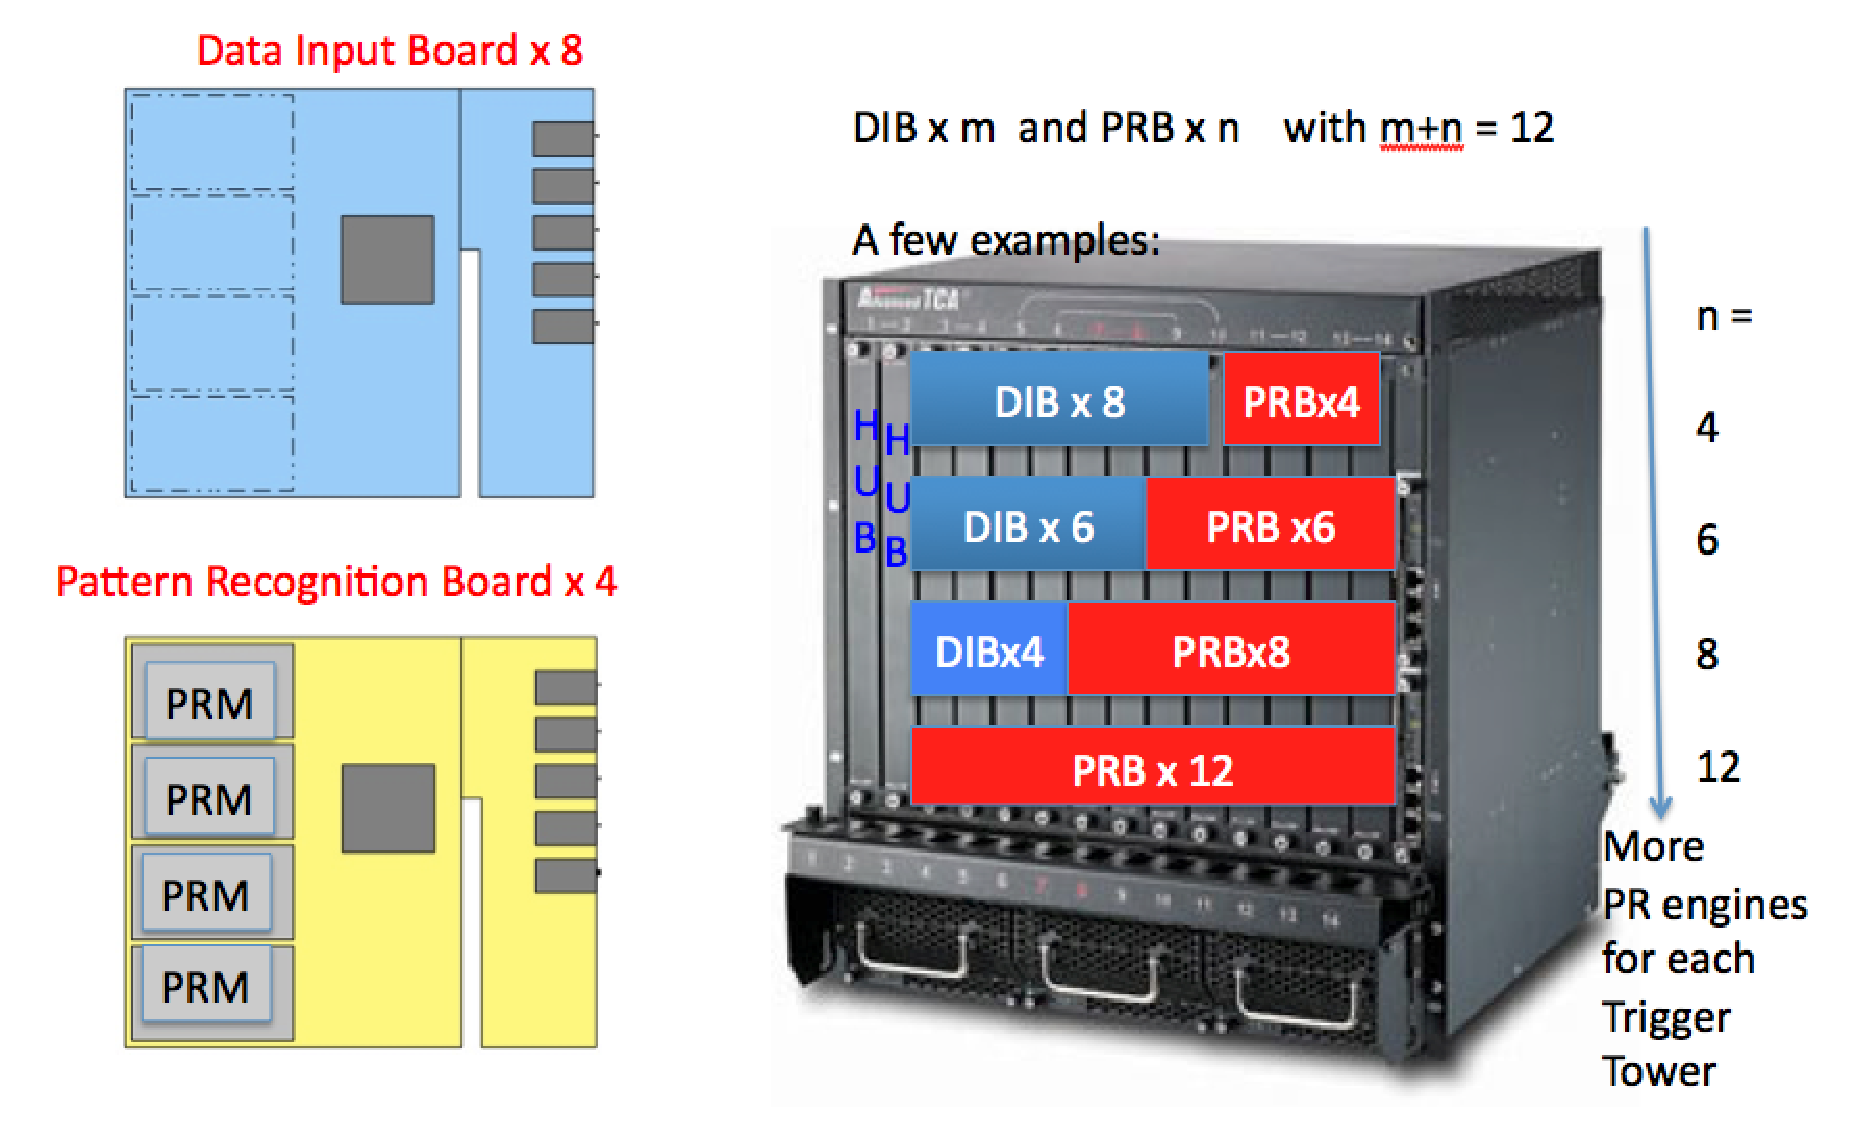
\includegraphics[width=0.7\columnwidth]{Plots/System_3.eps}
%\caption{System flexibility: many configurations possible \& being studied to select the right one for %demonstration purpose}
%\label{fig:System_3}
%\end{figure}


%\begin{table}[ht!]
%\centering\begin{tabular}{|c|c|c|c|c|}
%\hline
%DIB/PRB/PRM Count &  Fabric Channel BW (minimum)  &	PRM Input BW (minimum) \\
%8/4/16 &	20 Gbps &	40 Gbps \\
%6/6/24 &	20 Gbps &	27 Gbps \\
%4/8/32 &	20 Gbps &	20 Gbps \\
%\hline
%\end{tabular}
%\caption{Data sharing between towers occurs on the PRB board level.  Each PRB connects to the %corresponding PRB in the eight nearest tower processor shelves.  The above numbers assume a worst case %scenario of 500 32-bit stubs per trigger tower per event (every 25 ns).  An example of special configuration %with eight DIBs and four PRBs will be used as a simple example in Section 3.}
%\label{tab:shelves}
%\end{table}


\paragraph{DIB/PRB combo configuration}



%\begin{figure}[ht!]
%\centering
%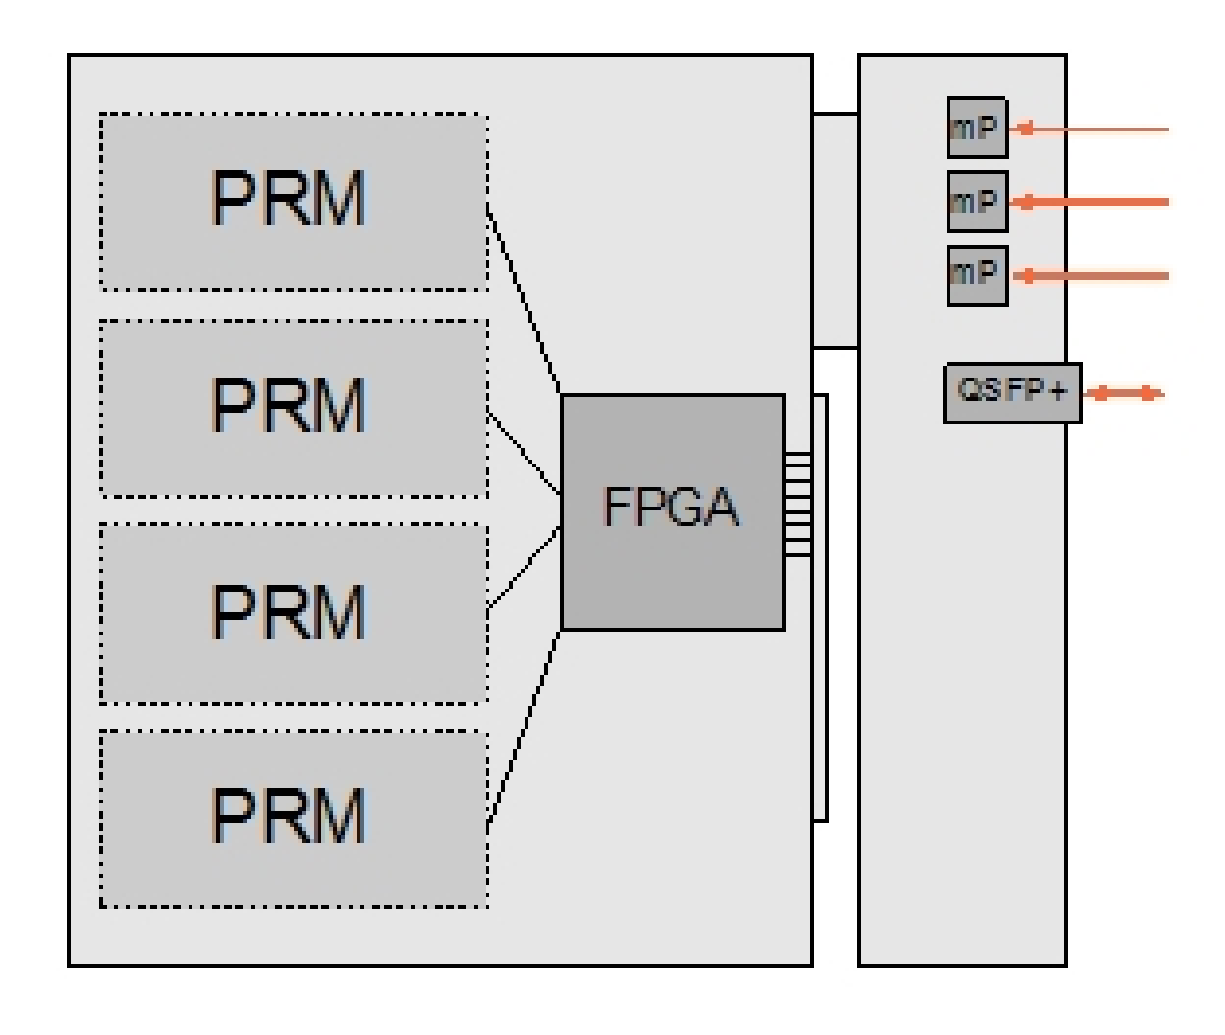
\includegraphics[width=0.45\columnwidth]{Plots/CombBlade.eps}
%\caption{Combined blade design}
%\label{fig:CombBlade}
%\end{figure}

\noindent DIB and PRB functionalities could also be combined into a single blade design, which is a special case of the "N DIB and M PRB" configuration described above (N=0 and M=12). A tower shelf would then consist of 10 Processor blades, one Gateway blade (for data sharing), and one Collector blade (for tracks found). These three different blade functionalities can be implemented in the same hardware, and Pulsar 2b is designed to meet all the requirements. The 10 Processor blades will process events in a round-robin fashion by  communicating over all available channels of the full-mesh backplane.
By using the full mesh fabric more effectively we are able to decrease the channel bandwidth requirement from 20 Gbps down to 6 Gbps with no significant latency increase. Note that Pulsar 2b has 20 Gbps fabric interface bandwidth capability, and therefore can meet the requirements in any of the system configurations described above.  


%\begin{figure}[ht!]
%\centering
%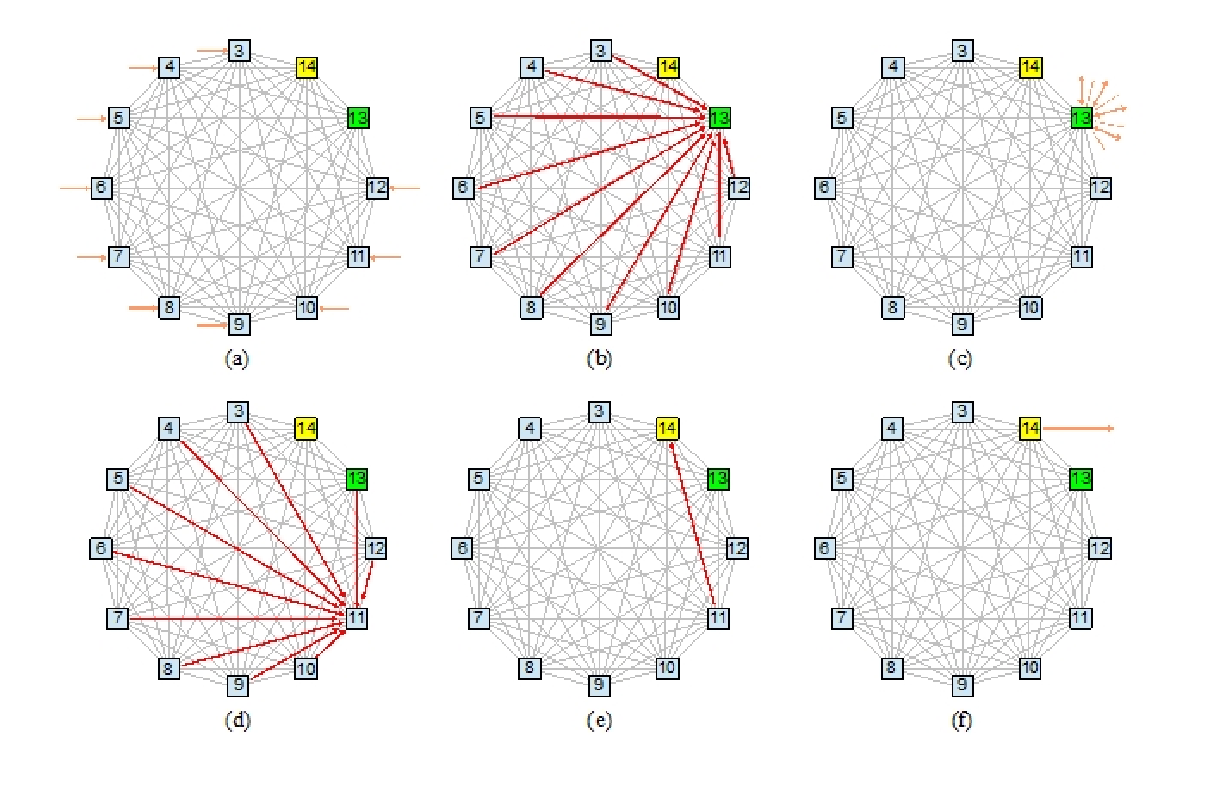
\includegraphics[width=0.9\columnwidth]{Plots/BackPlaneTr.eps}
%\caption{Backplane transfers sequences using the combined blade design. First, the input fibers are received %on the Processor blades (a).  Each Processor blade then transfers a portion of the input data to the Gateway %blade (b), where it is exchanged with neighboring towers over fiber links (c).  The Processor blades and %Gateway blade transfer the event (including neighbor data) to the target Processor blade in a time %multiplexed, round robin scheme (d).   Results from the Processor blades are then transferred to the %Collector blade (e) for any final formatting and processing before transmission downstream (f).}
%\label{fig:BackPlaneTr}
%\end{figure}
 

